\PassOptionsToPackage{unicode=true}{hyperref} % options for packages loaded elsewhere
\PassOptionsToPackage{hyphens}{url}
%
\documentclass[
]{article}
\usepackage{lmodern}
\usepackage{amssymb,amsmath}
\usepackage{ifxetex,ifluatex}
\ifnum 0\ifxetex 1\fi\ifluatex 1\fi=0 % if pdftex
  \usepackage[T1]{fontenc}
  \usepackage[utf8]{inputenc}
  \usepackage{textcomp} % provides euro and other symbols
\else % if luatex or xelatex
  \usepackage{unicode-math}
  \defaultfontfeatures{Scale=MatchLowercase}
  \defaultfontfeatures[\rmfamily]{Ligatures=TeX,Scale=1}
\fi
% use upquote if available, for straight quotes in verbatim environments
\IfFileExists{upquote.sty}{\usepackage{upquote}}{}
\IfFileExists{microtype.sty}{% use microtype if available
  \usepackage[]{microtype}
  \UseMicrotypeSet[protrusion]{basicmath} % disable protrusion for tt fonts
}{}
\makeatletter
\@ifundefined{KOMAClassName}{% if non-KOMA class
  \IfFileExists{parskip.sty}{%
    \usepackage{parskip}
  }{% else
    \setlength{\parindent}{0pt}
    \setlength{\parskip}{6pt plus 2pt minus 1pt}}
}{% if KOMA class
  \KOMAoptions{parskip=half}}
\makeatother
\usepackage{xcolor}
\IfFileExists{xurl.sty}{\usepackage{xurl}}{} % add URL line breaks if available
\IfFileExists{bookmark.sty}{\usepackage{bookmark}}{\usepackage{hyperref}}
\hypersetup{
  pdftitle={Copenhagen, Denmark},
  pdfauthor={Keene Morrow},
  pdfborder={0 0 0},
  breaklinks=true}
\urlstyle{same}  % don't use monospace font for urls
\usepackage[margin=1in]{geometry}
\usepackage{graphicx,grffile}
\makeatletter
\def\maxwidth{\ifdim\Gin@nat@width>\linewidth\linewidth\else\Gin@nat@width\fi}
\def\maxheight{\ifdim\Gin@nat@height>\textheight\textheight\else\Gin@nat@height\fi}
\makeatother
% Scale images if necessary, so that they will not overflow the page
% margins by default, and it is still possible to overwrite the defaults
% using explicit options in \includegraphics[width, height, ...]{}
\setkeys{Gin}{width=\maxwidth,height=\maxheight,keepaspectratio}
\setlength{\emergencystretch}{3em}  % prevent overfull lines
\providecommand{\tightlist}{%
  \setlength{\itemsep}{0pt}\setlength{\parskip}{0pt}}
\setcounter{secnumdepth}{-2}
% Redefines (sub)paragraphs to behave more like sections
\ifx\paragraph\undefined\else
  \let\oldparagraph\paragraph
  \renewcommand{\paragraph}[1]{\oldparagraph{#1}\mbox{}}
\fi
\ifx\subparagraph\undefined\else
  \let\oldsubparagraph\subparagraph
  \renewcommand{\subparagraph}[1]{\oldsubparagraph{#1}\mbox{}}
\fi

% set default figure placement to htbp
\makeatletter
\def\fps@figure{htbp}
\makeatother


\title{Copenhagen, Denmark}
\usepackage{etoolbox}
\makeatletter
\providecommand{\subtitle}[1]{% add subtitle to \maketitle
  \apptocmd{\@title}{\par {\large #1 \par}}{}{}
}
\makeatother
\subtitle{ESM 327 Homework \#1 - Climate Trends}
\author{Keene Morrow}
\date{4/15/2020}

\begin{document}
\maketitle

\hypertarget{background}{%
\paragraph{Background}\label{background}}

Copenhagen is the capital of Denmark. Located on the east side of
Denmark's largest island, Zealand, Copenhagen is separated from Sweden
by the Øresund. In the author's experience, the city is dominated by
paved areas but has numerous parks and easy access to the harbor for
recreation. Topographically, the city, like the rest of Denmark, is
remarkably flat.

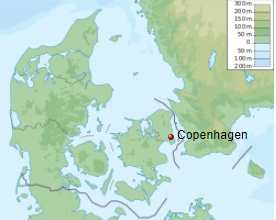
\includegraphics{figures/kbh.png} \emph{Copenhagen's location within
Denmark. Source: Wikipedia}

As a coastal city, Copenhagen is particularly vulnerable to sea level
rise and coastal flooding. Local fisheries will be impacted by the shift
of marine species towards higher latitudes. Changes in precipitation and
the exacerbation of extreme weather may impact agriculture in the area,
both positively (increased cereal yields, possibility of wine grape
cultivation) and negatively (increased pest activity, impact of heat on
livestock). Extreme heat and cold are expected to have significant
socioeconomic and health effects. (IPCC 2014)

\hypertarget{data}{%
\paragraph{Data}\label{data}}

Data from the Danish Meterological Institute (Danmarks Meteorologiske
Institut) meteorological station at Landbohøjskolen, Københavns
Universitet (Land High School, University of Copenhagen) will be used to
assess the climate trends from January 1, 1874 and December 31, 2019.
The precipitation data contained 44834 daily observations. No data was
available for 272 days within the observation period. The temeprature
data contained 106557 daily high and low observations. No data was
available for 95 days within the observation period.

\hypertarget{analysis}{%
\paragraph{Analysis}\label{analysis}}

Annual and decadal deviation from the 20th century average were
calculated for both temperature and precipitation. Temperature deviation
increases through time, with more deviation in daily low temperatures.
While days in Copenhagen are getting warmer, nights are getting hotter.
(Figure 1) Only a slight upward trend after 1960 emerges from the same
analysis of precipitation (Figure 2)

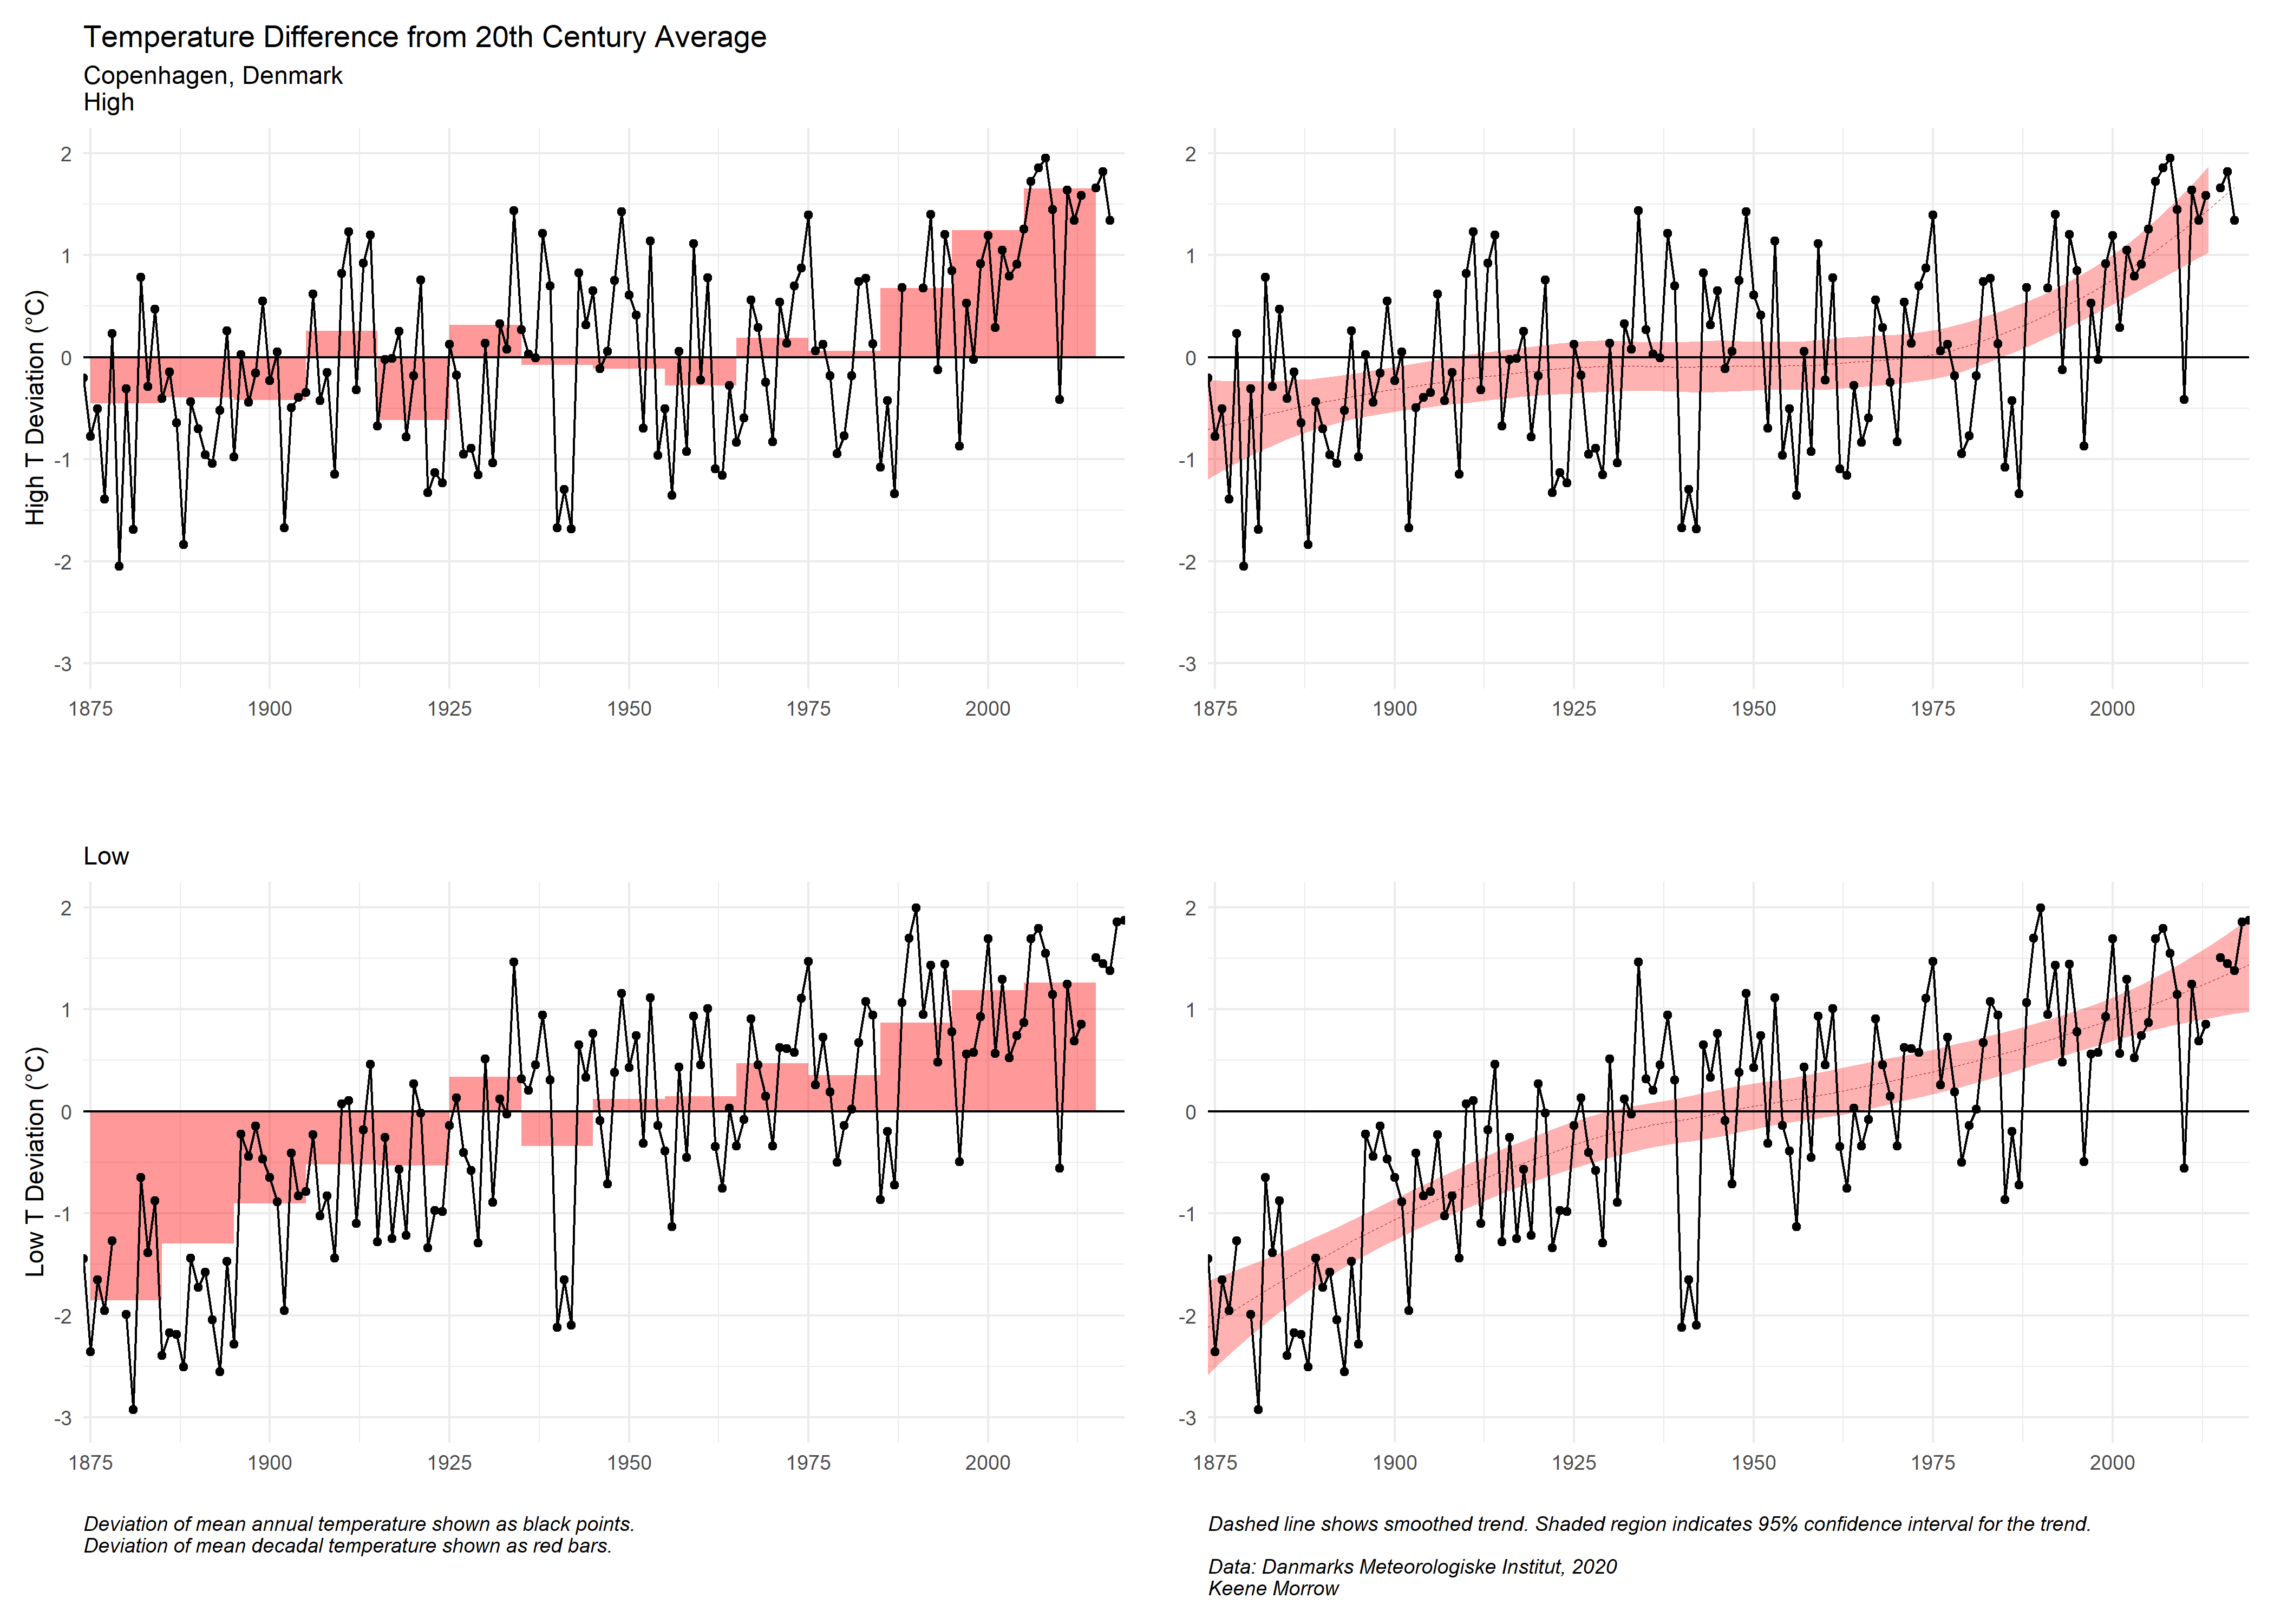
\includegraphics{figures/temp_dev_20.png} \emph{Figure 1}

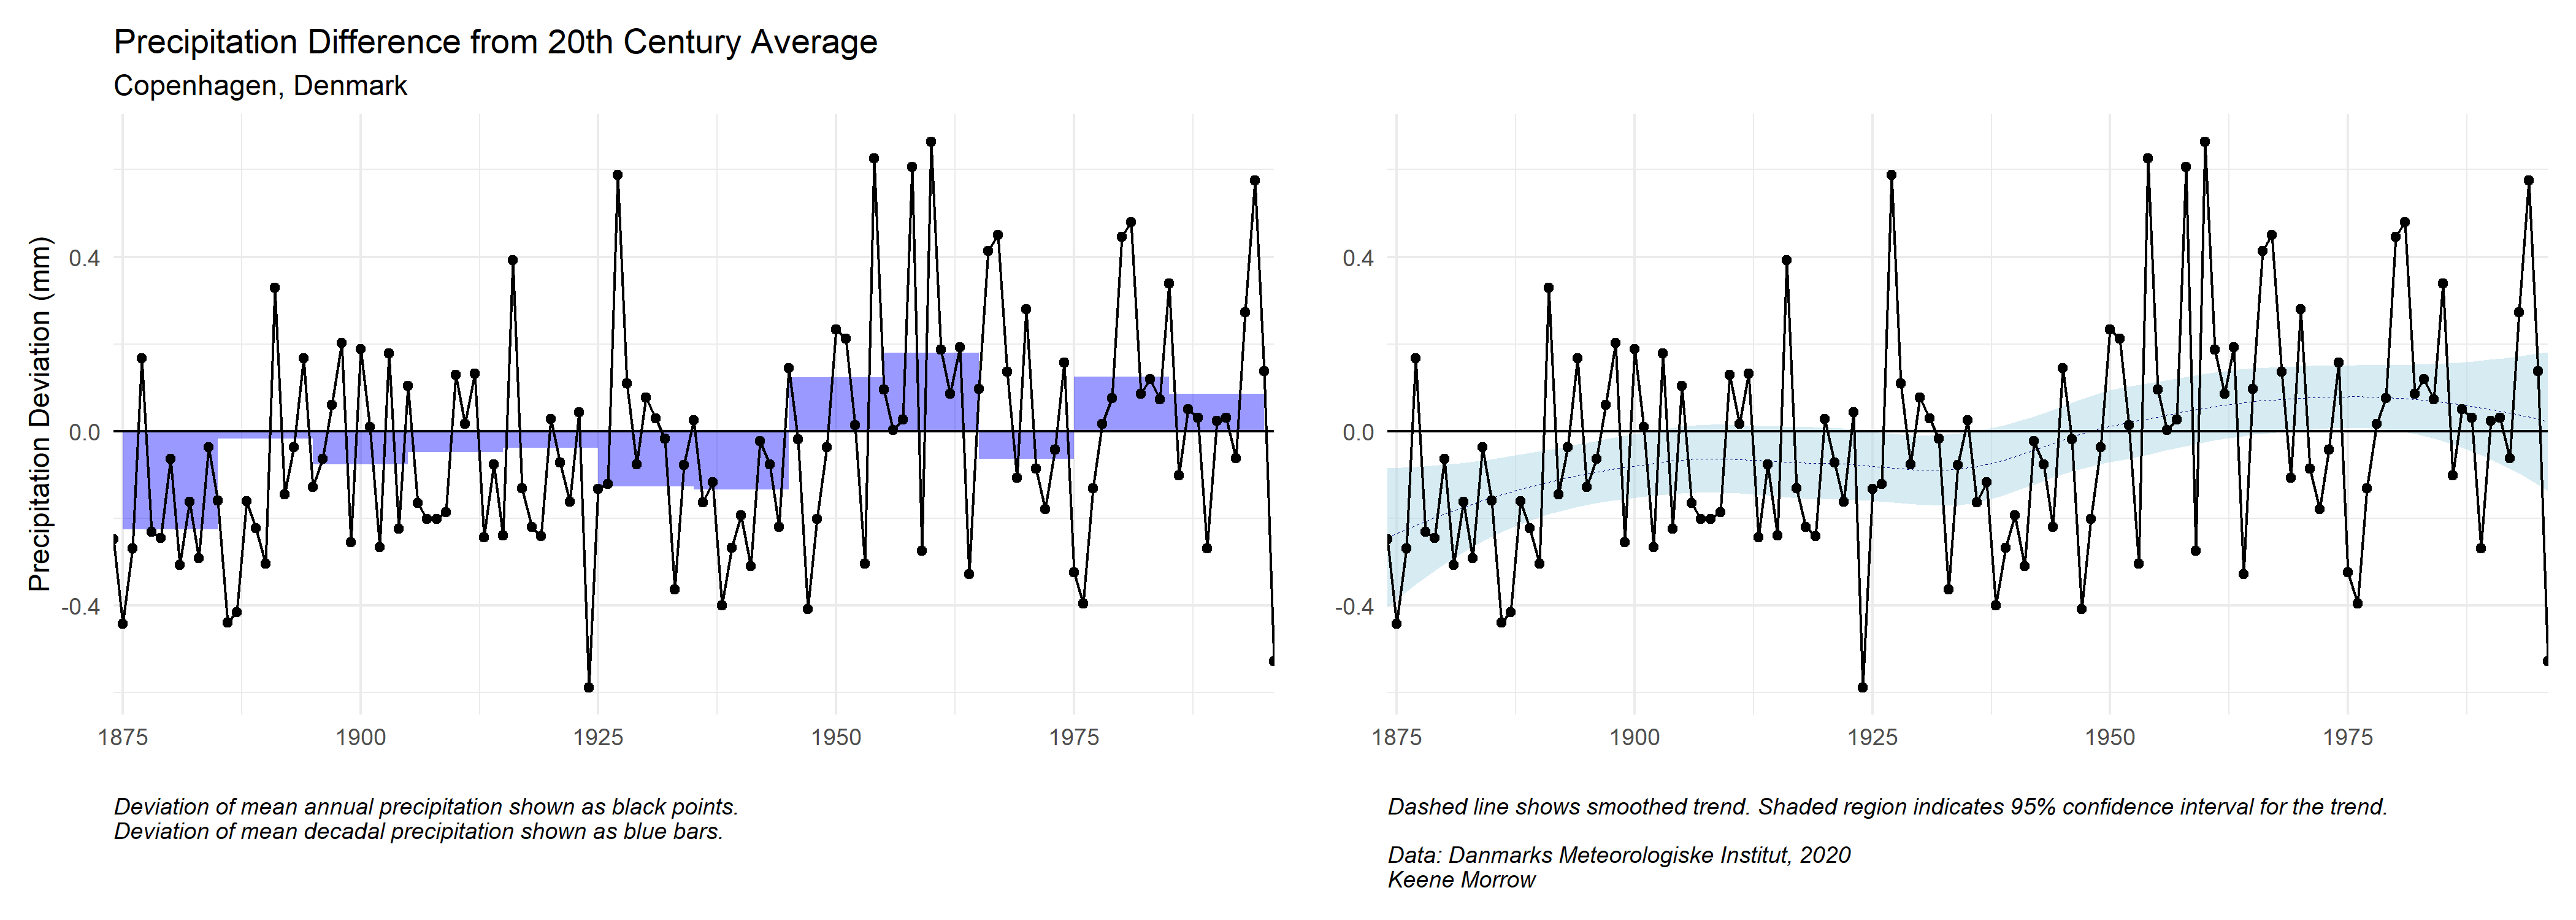
\includegraphics{figures/precip_dev_20.png} \emph{Figure 2}

The reduction in daily temperatures is reflected in the number of frost
days over time. A decline is noticable throughout the observation
period, with a more rapid decline in before 1925 and after 1975. (Figure
3) Fewer frost days may cause an increase in agricultural pests in the
region due to decrease die offs from freezing temepratures.

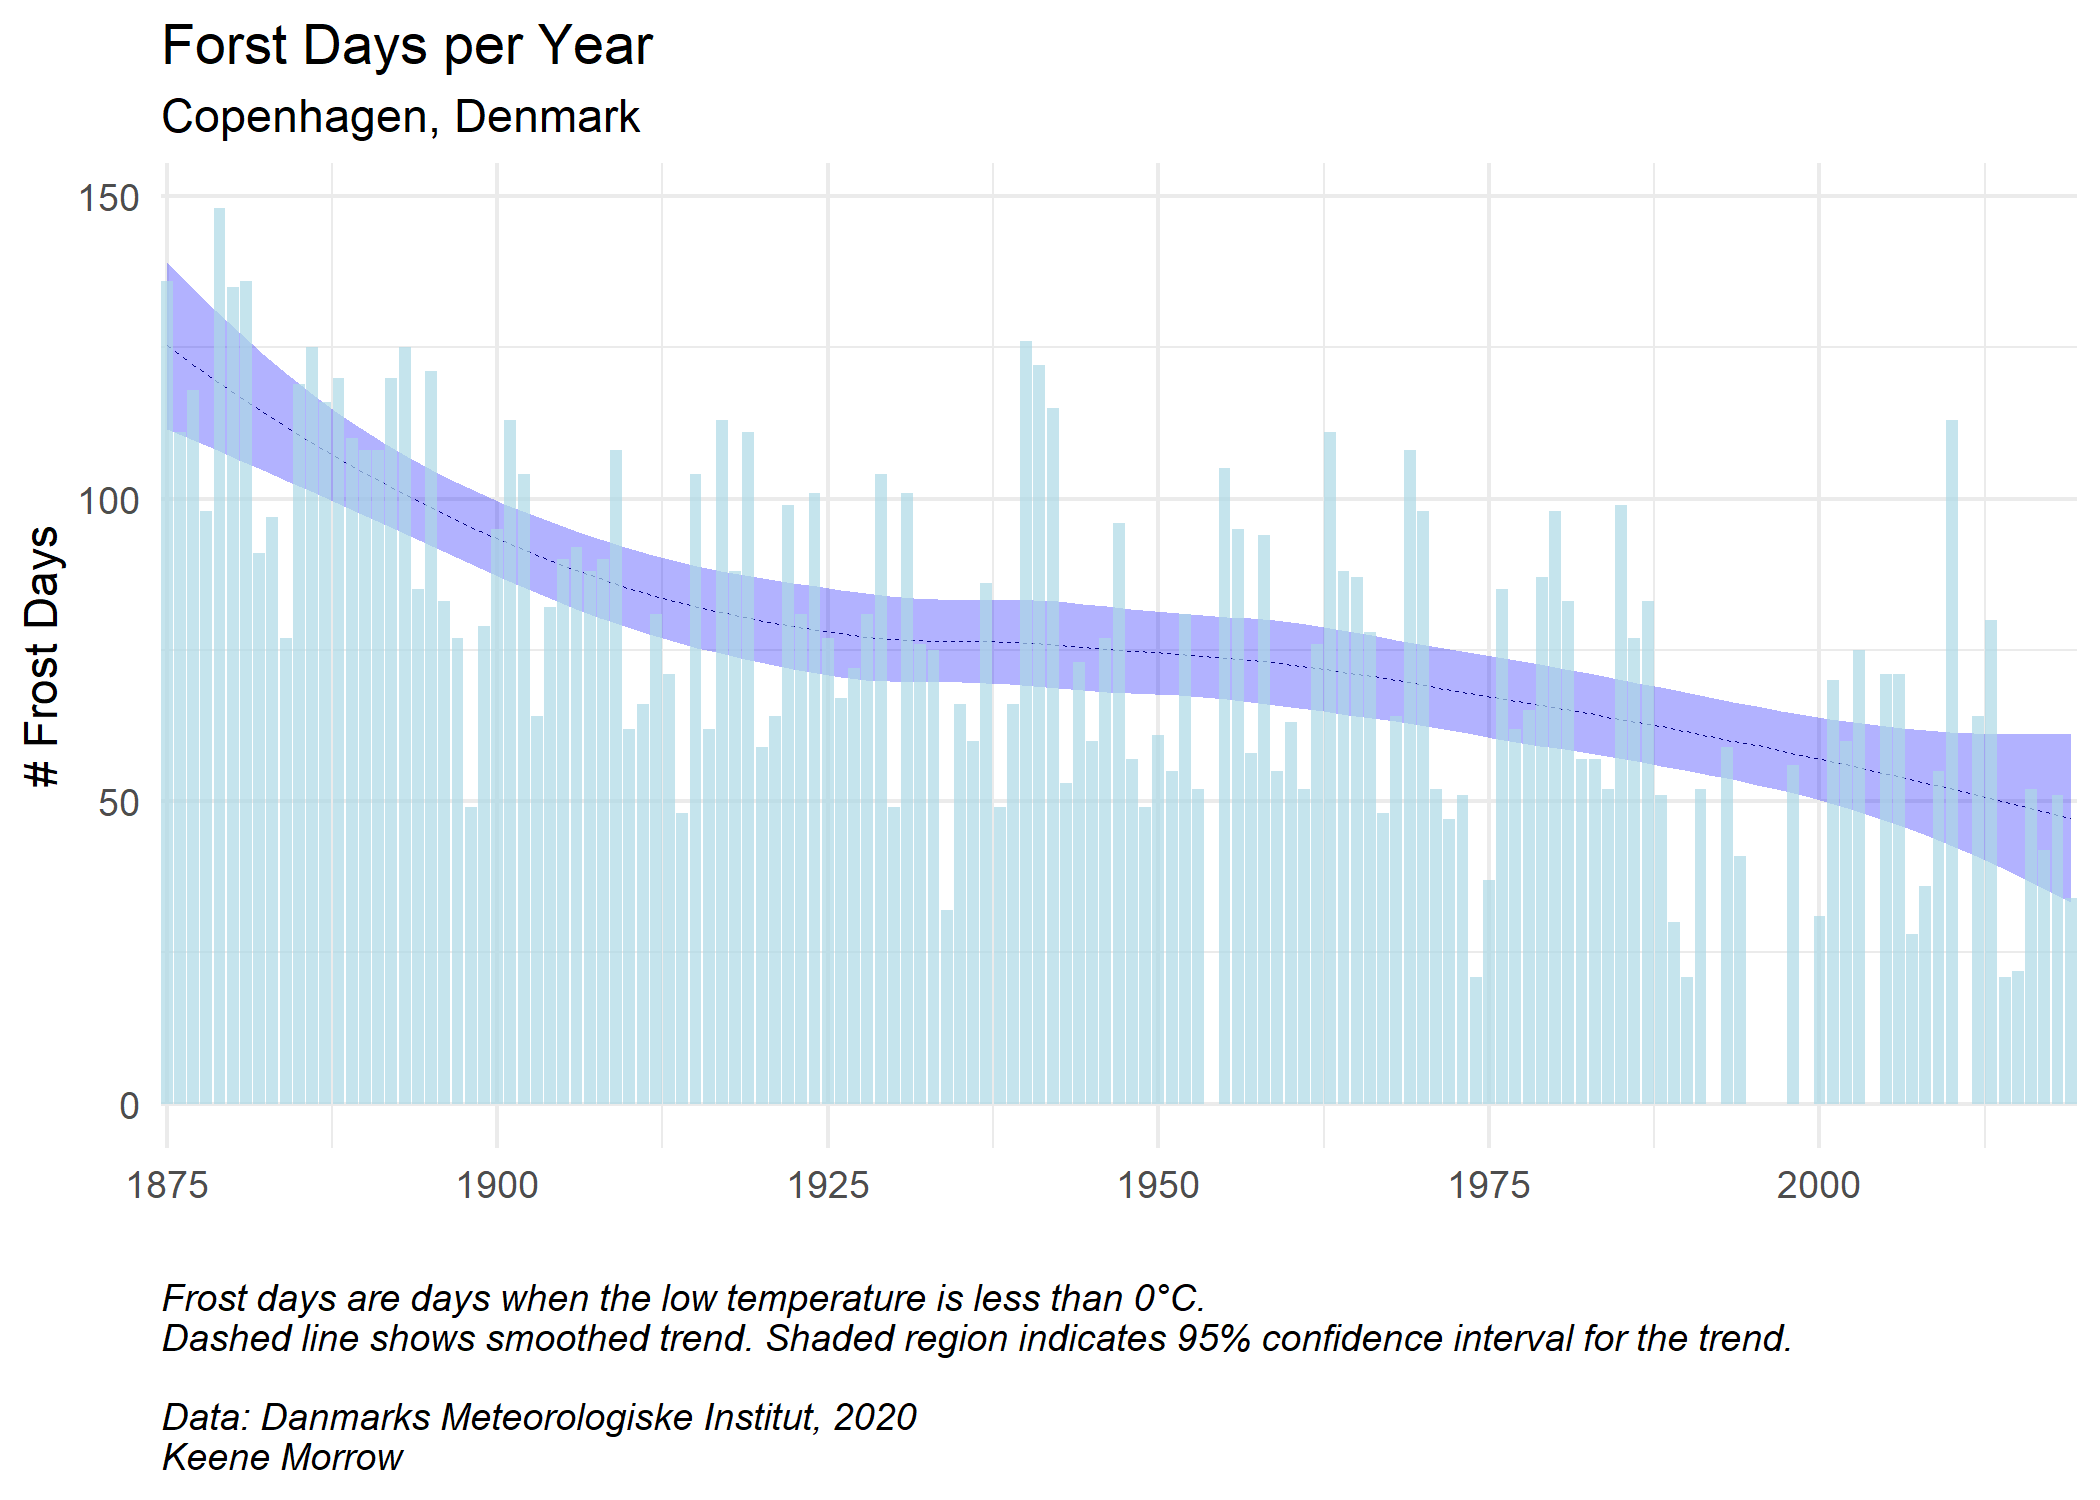
\includegraphics{figures/frost_days.png} \emph{Figure 3}

An examination of changes in seasonal mean high temperature show that
the greatest impacts to temperature can be seen during the winter,
spring, and fall. Lows, by contrast, follow similar upward trends
regardless of season. (Figure 4) This suggests that extreme heat may not
be an immediate concern of those raising livestock. The concavity of the
trend in the hottest day of the year suggests that extreme heat may
become of increasing concern in the future. (Figure 5)

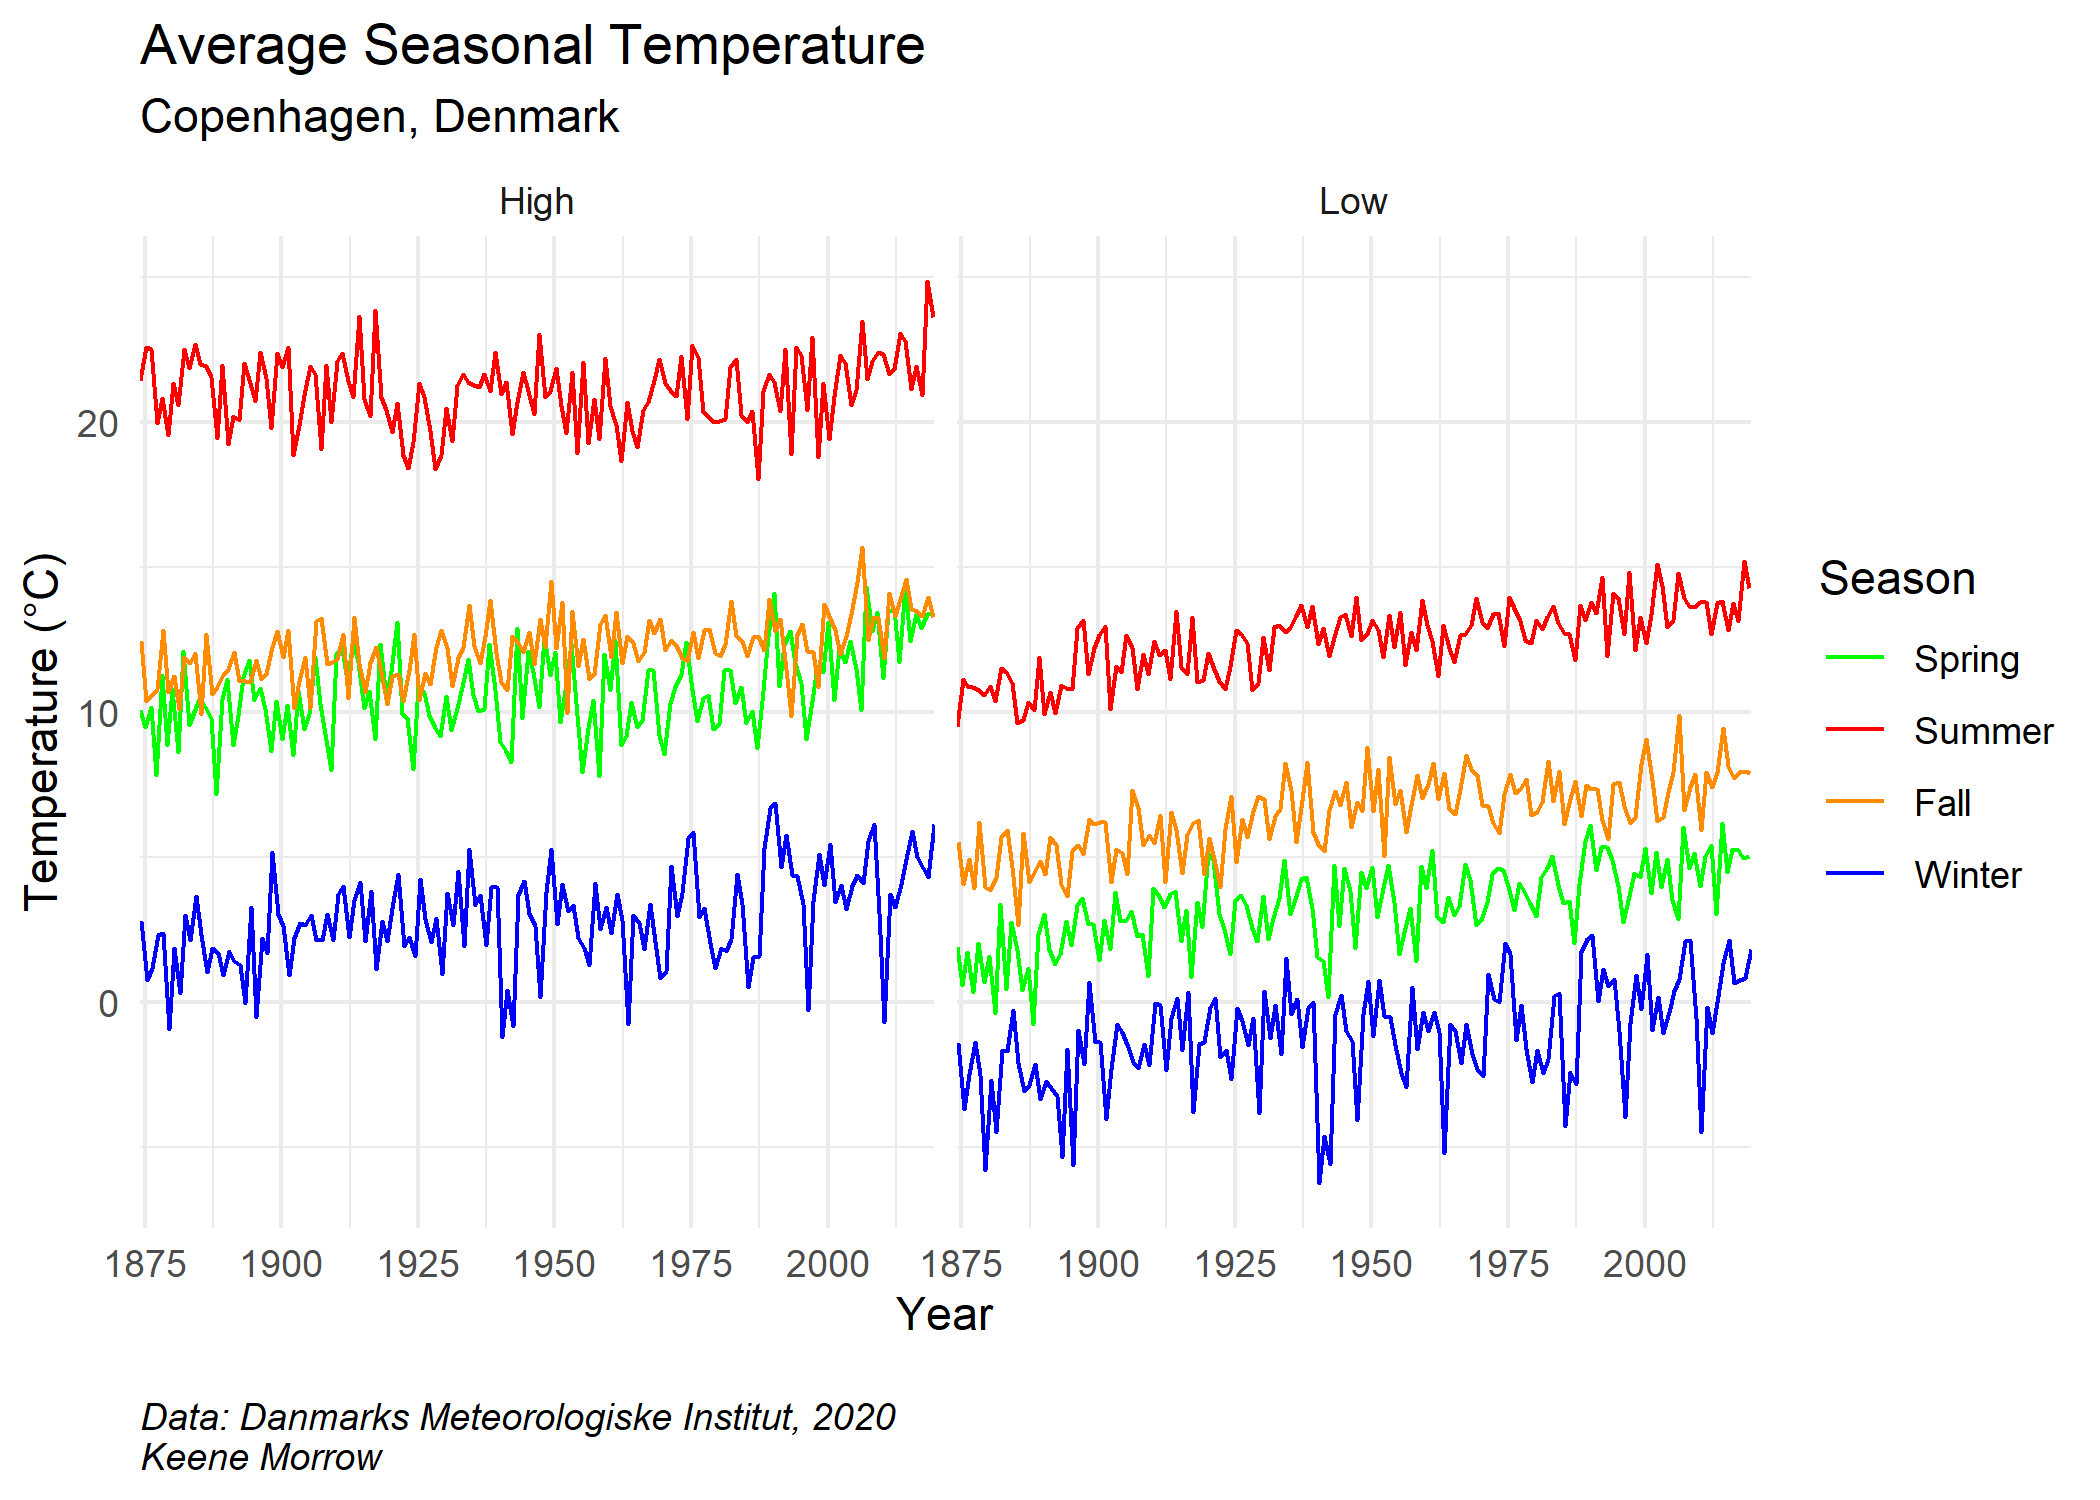
\includegraphics{figures/mean_season_temp.png} \emph{Figure 4}
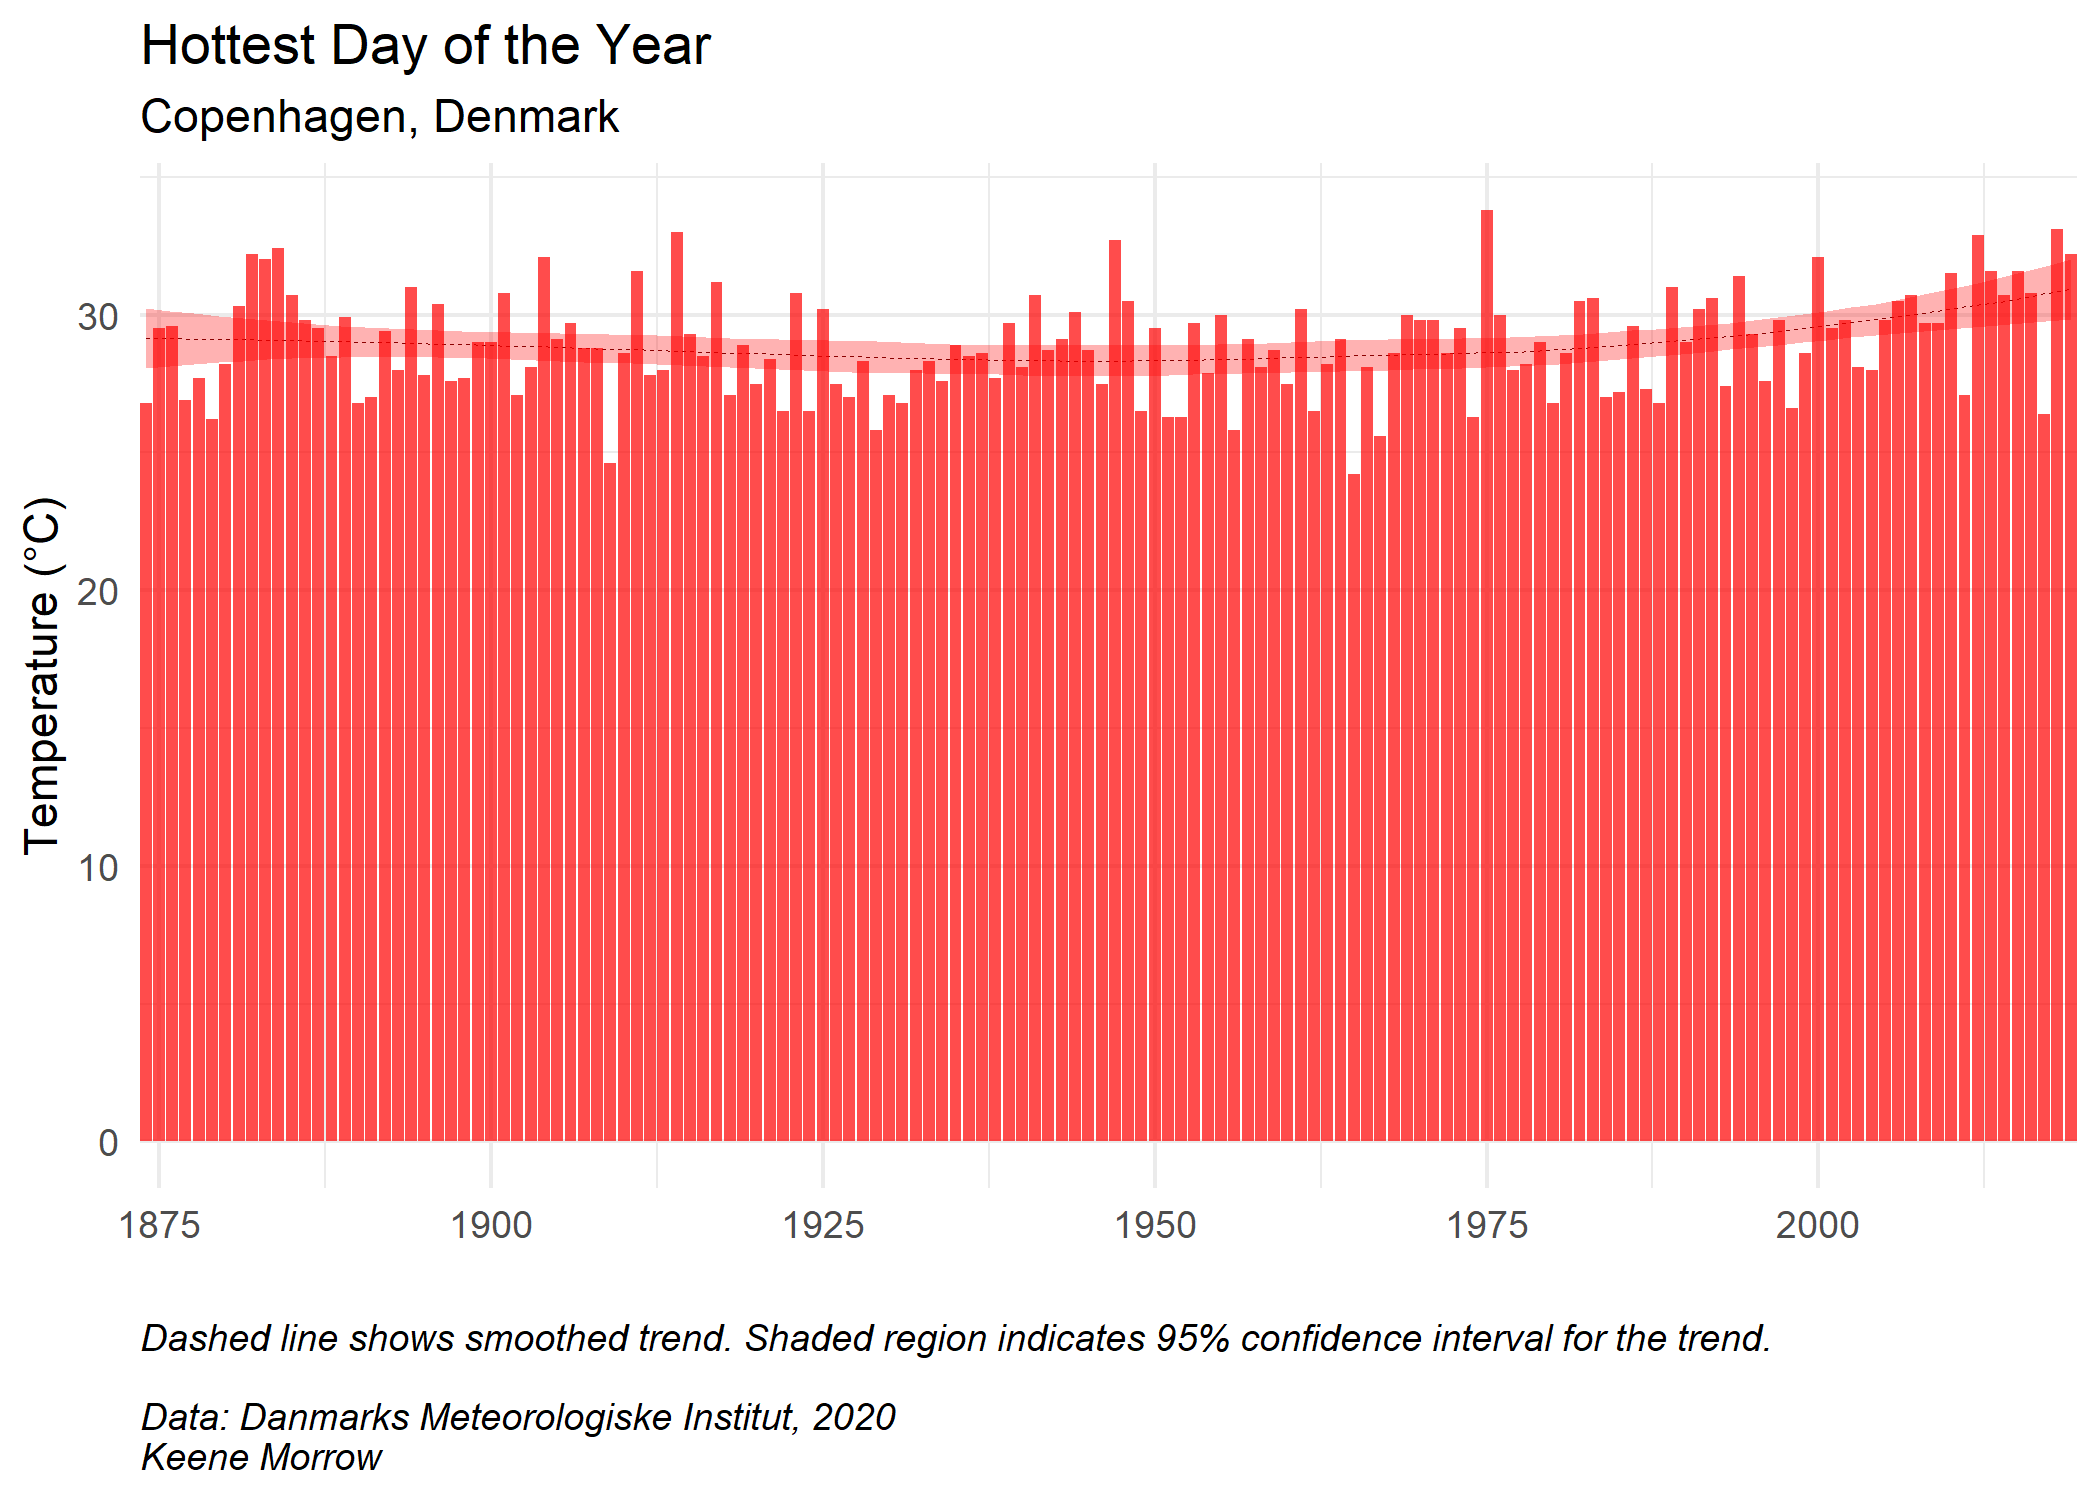
\includegraphics{figures/max_T.png} \emph{Figure 5}

Monthly mean temperatures (Figure 6) show the most deviation from
historic records in winter months, particularly in lows. Like other
metrics, monthly mean lows have seen more consistent elevation than
highs.

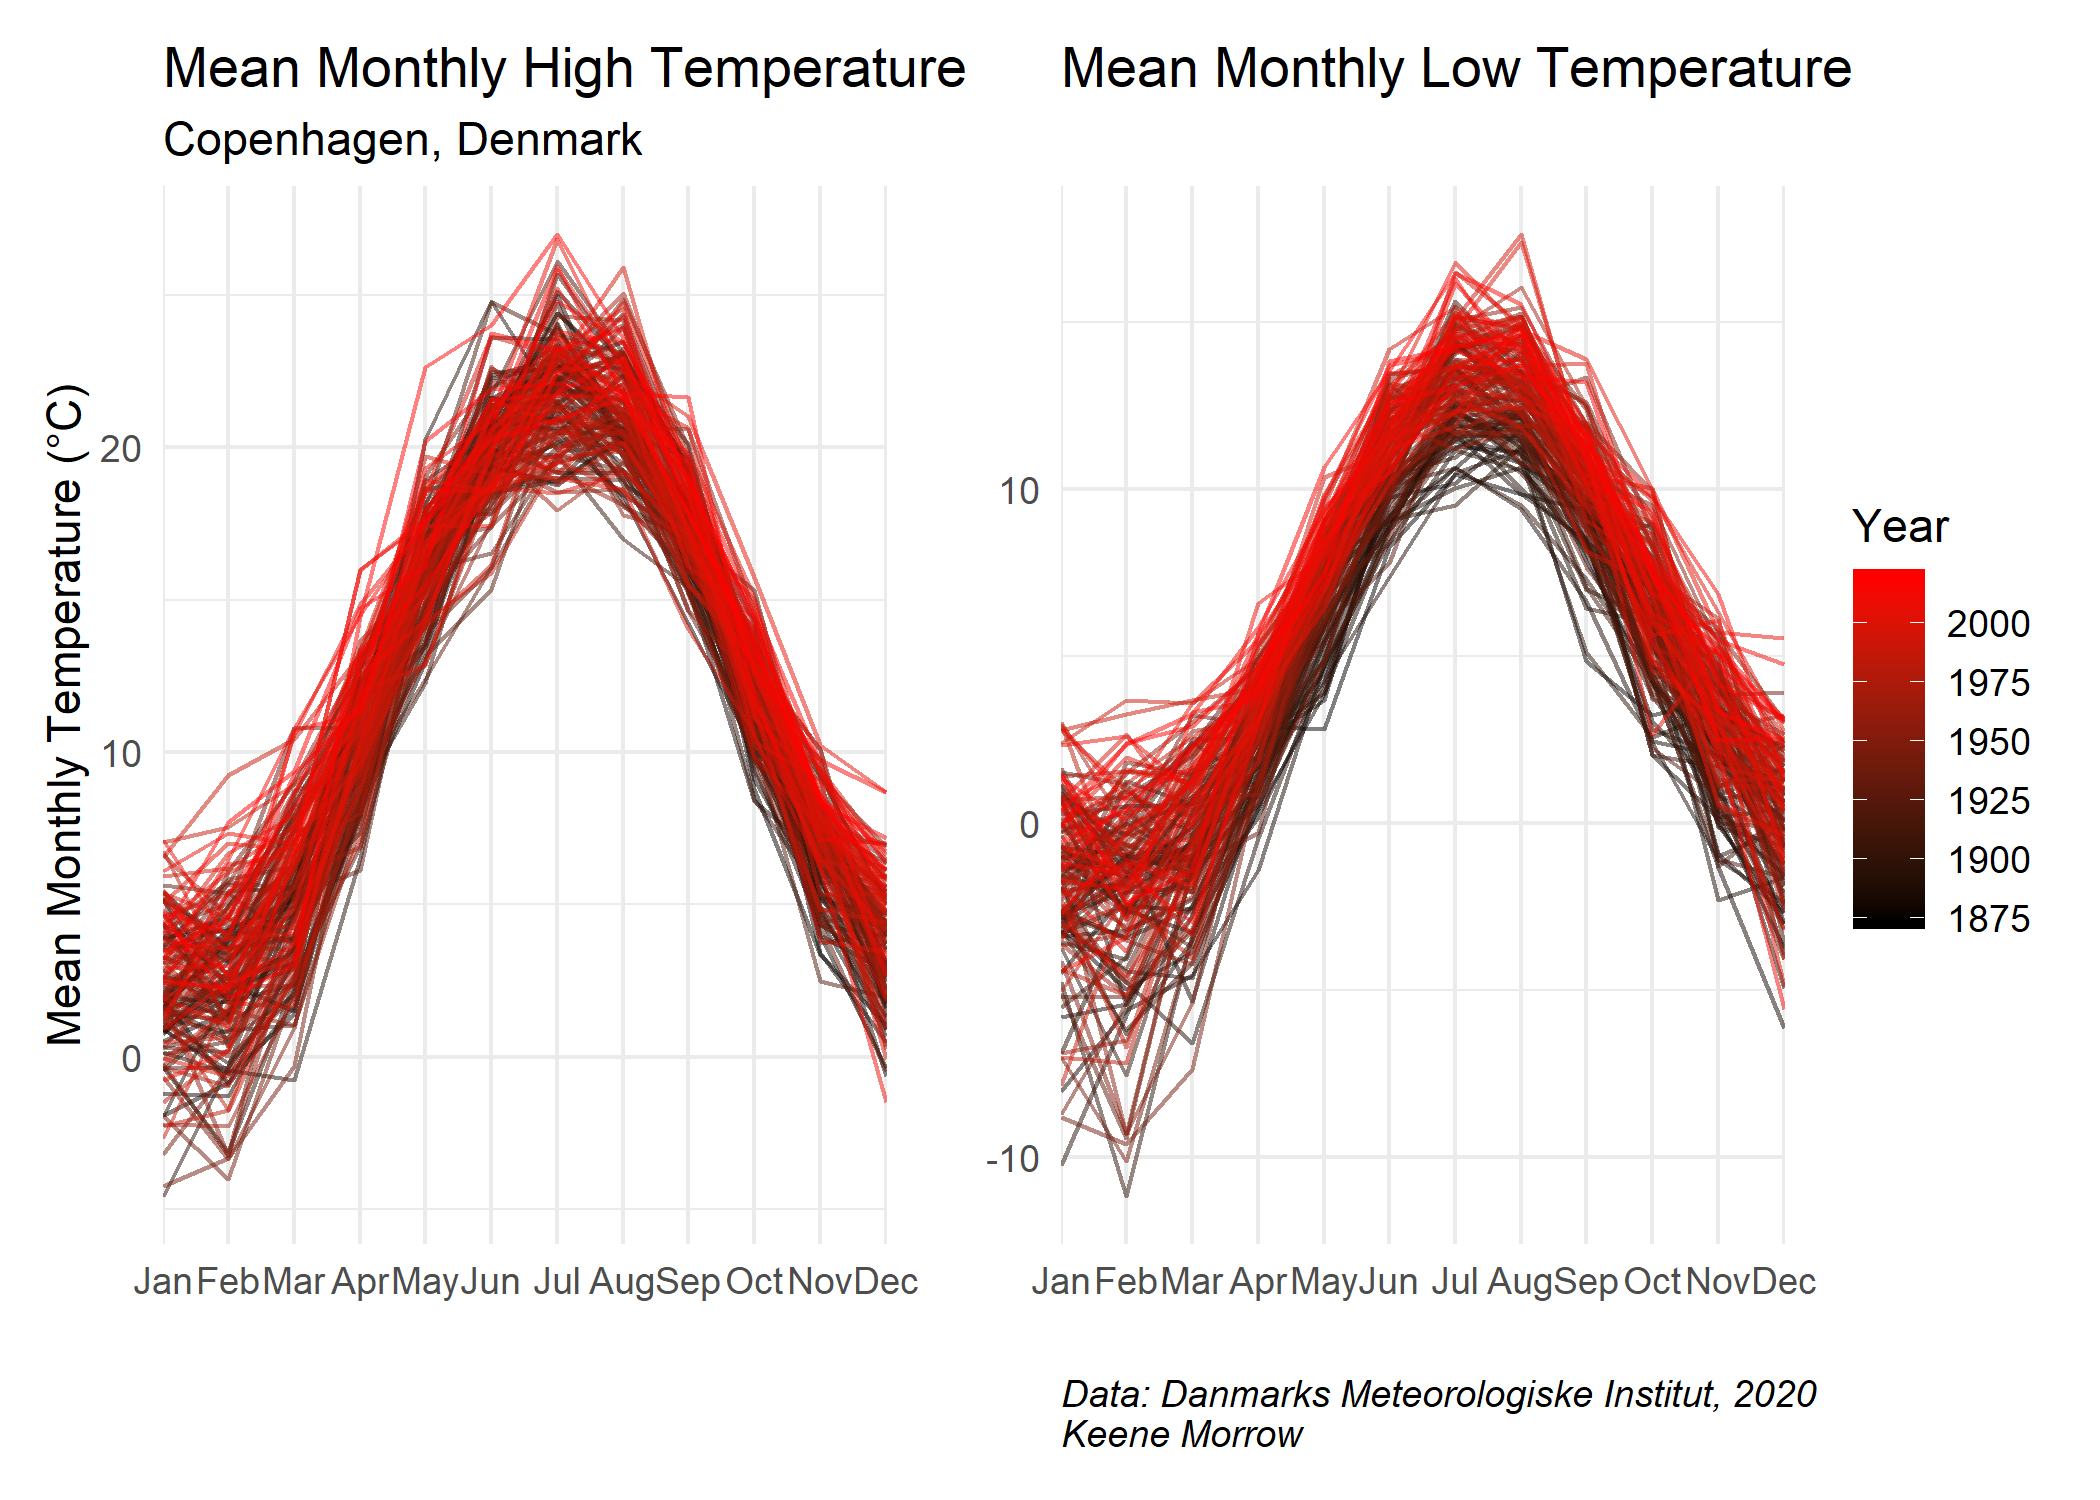
\includegraphics{figures/mean_month_temp.png} \emph{Figure 6}

Seasonal and monthly trends in precipitation are difficult to discern.
There may be a slight increase in spring precipitation. Other trends
could not be discerned. (Figures 7 \& 8)

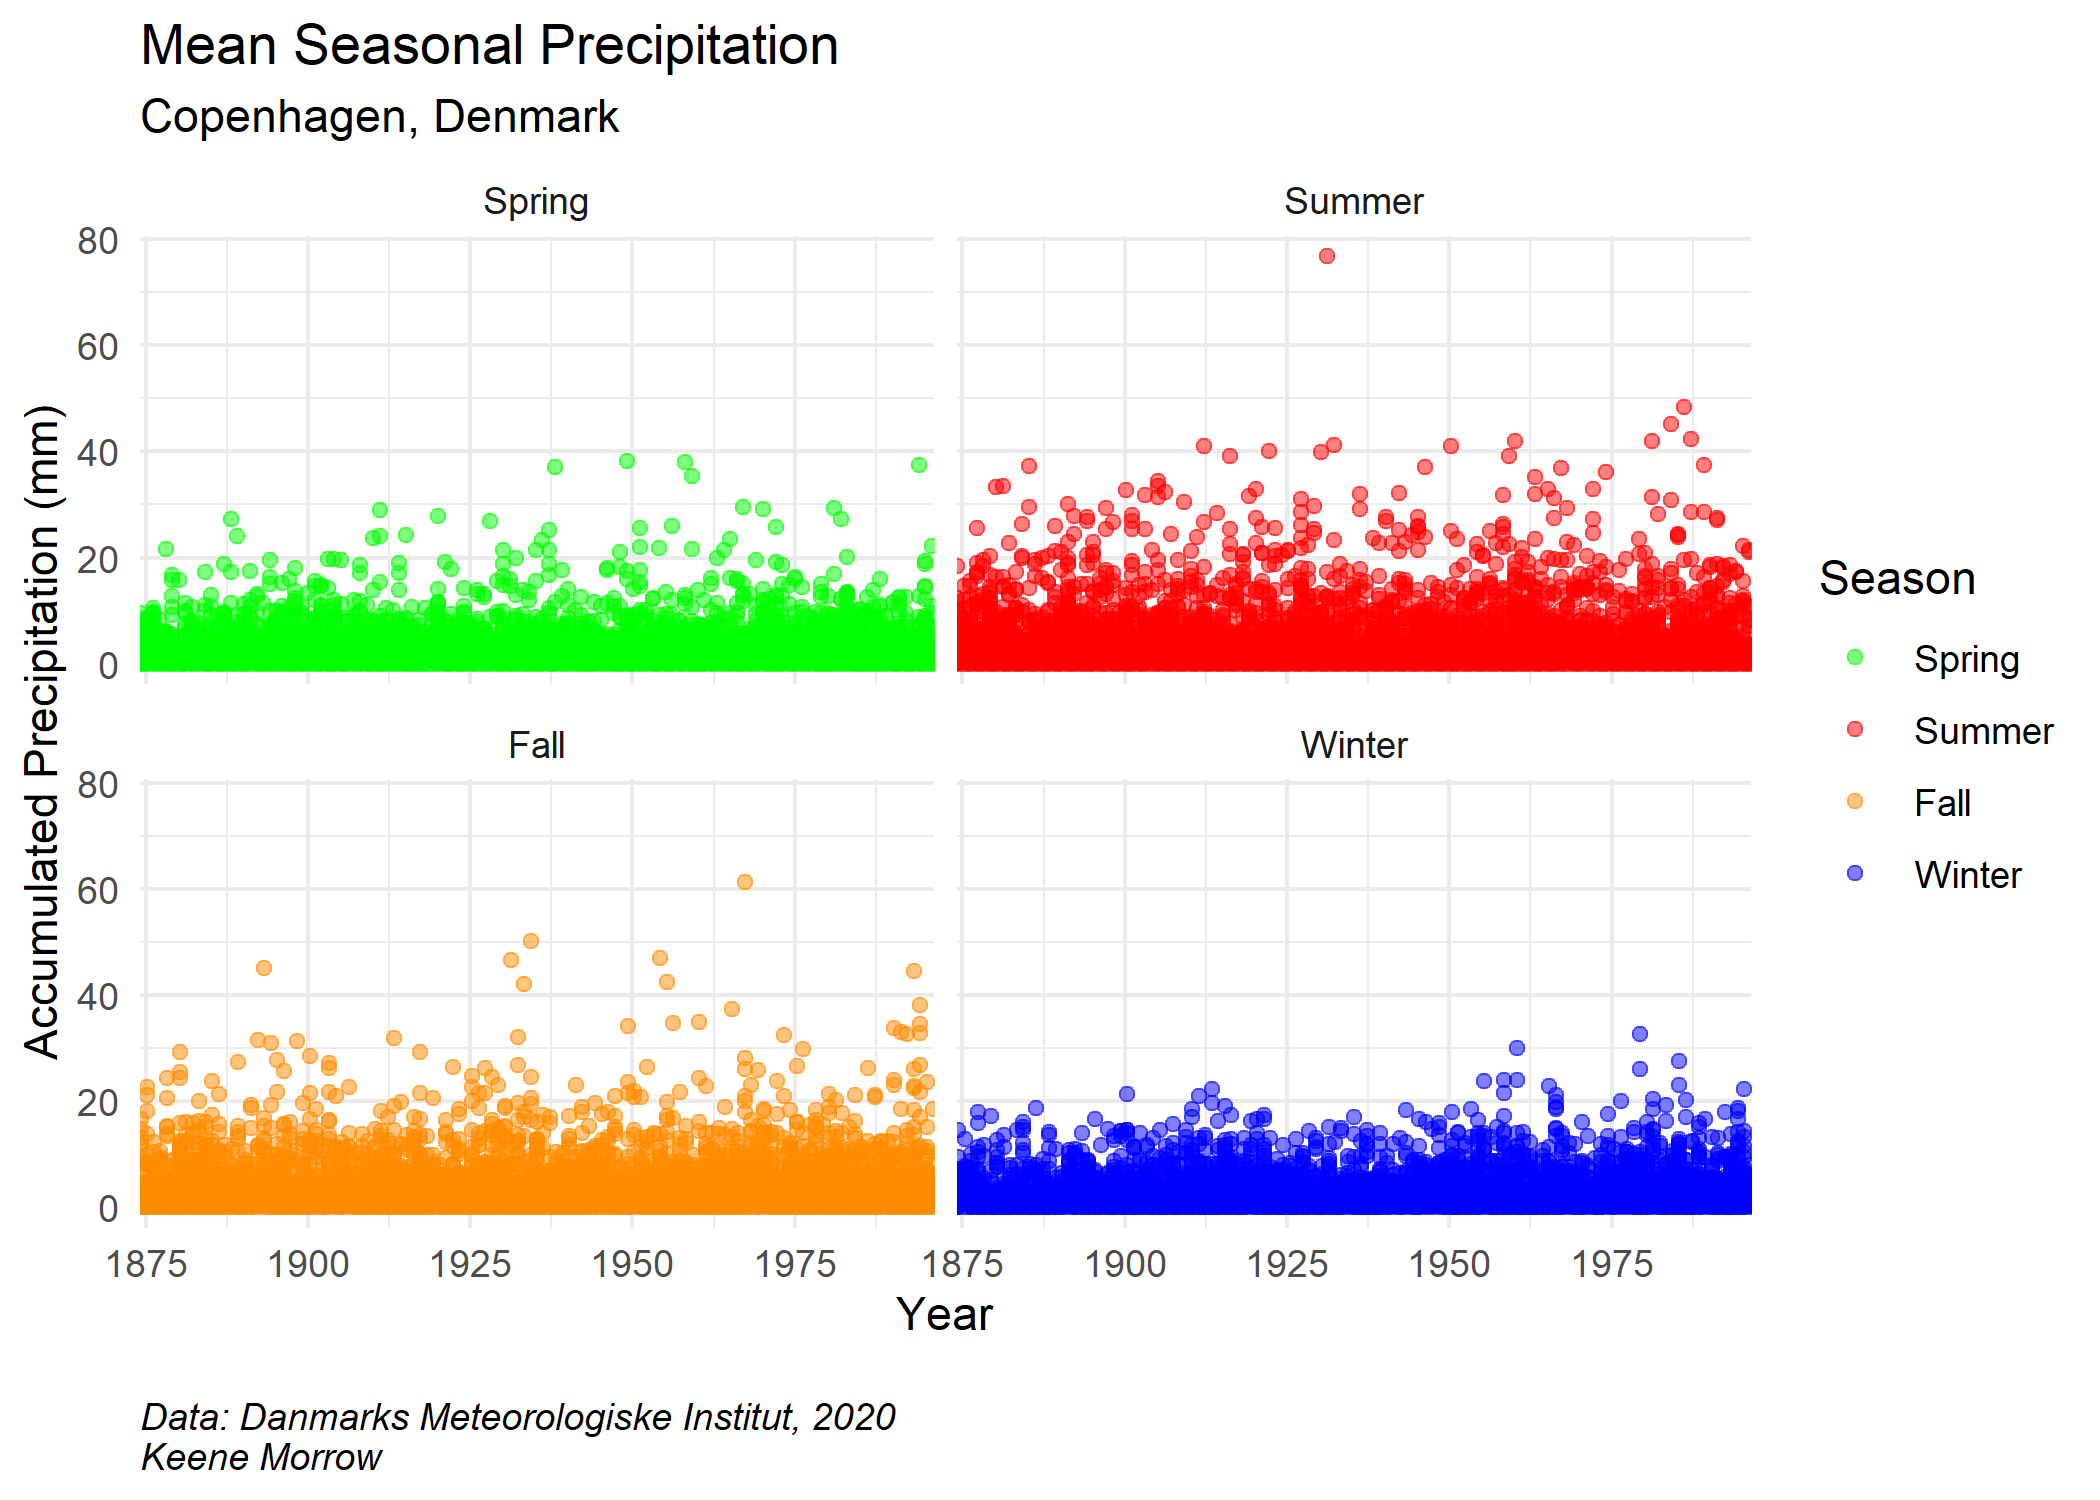
\includegraphics{figures/mean_season_precip.png} \emph{Figure 7}
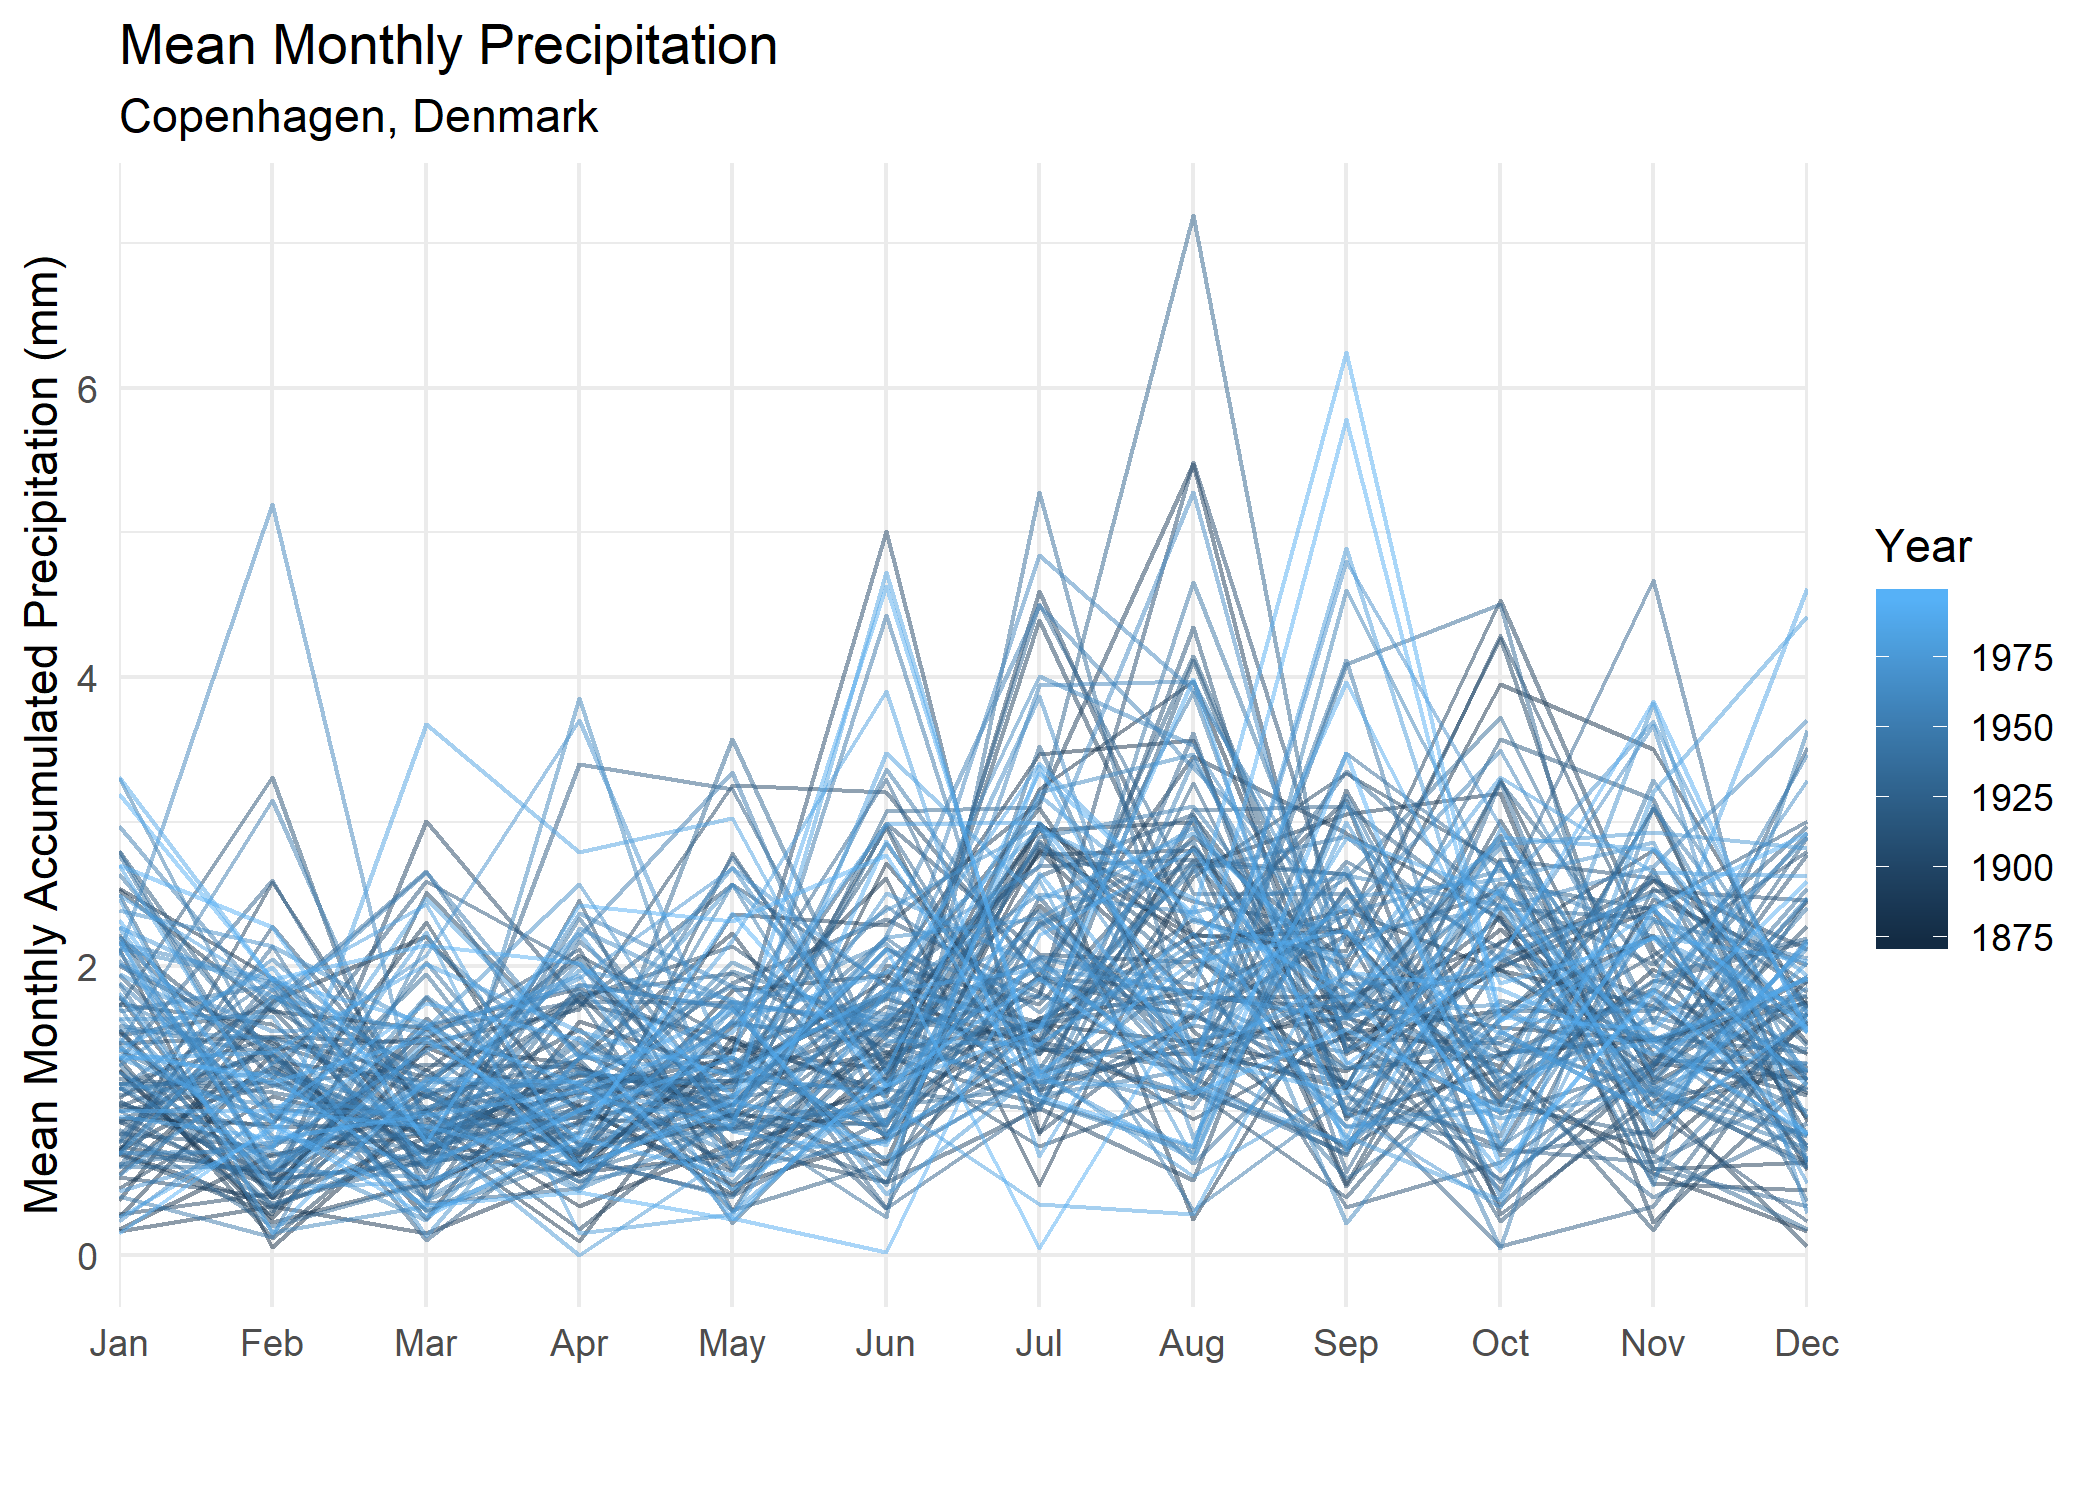
\includegraphics{figures/mean_month_precip.png} \emph{Figure 8}

\hypertarget{conclusion}{%
\paragraph{Conclusion}\label{conclusion}}

Copenhagen has historically benefited from a mild maritime climate.
Ocean warming may exacerbate existing upward trends in temperature,
especially lows. There has been little discernable change in
precipitation to date, but continued disruption to temperatures may
force more extreme increases in precipitation. These trends may
significantly impact agricultural systems in Denmark as a whole.

\begin{center}\rule{0.5\linewidth}{\linethickness}\end{center}

\hypertarget{references}{%
\paragraph{References}\label{references}}

IPCC, 2014. ``AR5 Climate Change 2014: Impacts, Adaptation, and
Vulnerability, Part B: Regional Aspects.''
\url{https://www.ipcc.ch/report/ar5/wg2/}

Cappelen, John. 2020. ``DMI Report 20-02 Denmark - DMI Historical
Climate Data Collection 1768-2019.'' Danmarks Meteorologiske Institut.
\url{https://www.dmi.dk/fileadmin/user_upload/Rapporter/TR/2020/DMIRep20-02.pdf}

\end{document}
